\section{Communication between the shell- and the remote-application}\label{section:applied-methods:communication-shell-remote}

The next step was to implement communication between the application shell and the micro-frontends. Apollo Client's cache should be used to increase the performance of the micro-frontend architecture. Therefore, the application shell and the micro-frontends must share the same instance of the in-memory cache. How the in-memory cache works is described in chapter  \ref{subsubsection:background:graphql:apollo-server-client:in-memory-cache-working}. The application shell must provide the cache instance to the micro-frontends to create a shared caching layer. The implementation details will be explained in section \ref{section:applied-methods:shared-caching-layer} in more detail. This section focuses on communication between the application shell and the micro-frontends.

\bigskip

\noindent To allow parallel development and deployment of micro-frontends, it is necessary that their implementation stays as independent as possible. Two micro-frontends should not communicate with each other directly, as it creates a tight coupling. Instead, it is better that one micro-frontend communicates to the other micro-frontends by publishing events to a central event bus, and the other micro-frontends subscribe to the events. This pattern is known as publish/subscribe mechanism. Alternatively, the application shell orchestrates the communication of the micro-frontends. One micro-frontend emits an event, and the application shell intercepts that. The application shell propagates the event to the target micro-frontend afterwards. This approach drastically reduces the coupling between micro-frontends. No micro-frontend needs information about the other remote applications, allowing for parallel development.

\bigskip

\noindent As explained in chapter \ref{subsection:background:micro-frontend:communication-patterns} three distinct types of communication exist between micro-frontends and the application shell. Angular provides an excellent feature for implementing unidirectional communication between micro-frontends, namely dependency injection. The application shell can provide services that remote applications can inject. An Angular injection token was created to implement specific behavior if an application runs in standalone mode or is consumed by an application shell.

\noindent An injection Token can be used to define a dependency that should be injectable into a class. An injection token can be of any value, but the injected type is usually not reified, which means that it is not available at runtime.\cite{misc:-:applied-methods:communication:angular-injection-token}

% TODO: explain injection-token in more detail

\bigskip

\noindent The following paragraph describes the usage of the token inside the contact application, but the usage is the same for every micro-frontend inside the architecture. The definition and the usage of the token is shown in the listing \ref{code:applied-methods:communication-patterns:providing-native-configuration}. The core module inside the contact application provides the token, which specifies that if the token can be injected, the application runs in standalone mode. The token is used by the contact's feature module, which is also the module that is exposed via Module Federation. The contact remote module injects the token to run additional logic if the application shell consumes it. The application shell does not need to provide the injection token because the logic is not executed if it is not defined.

\ifshowListings
  \begin{listing}[H]
  \begin{minted}{typescript}

const CONTACT_NATIVE_ENVIRONMENT = 
new InjectionToken<boolean>('CONTACT_NATIVE_ENVIRONMENT');

@NgModule({
  imports: [
    ...
  ],
  providers: [
    { provide: CONTACT_NATIVE_ENVIRONMENT, useValue: true },
  ]
})
class ContactCoreModule {}
  \end{minted}
  \caption{Providing the application with the native token.}\label{code:applied-methods:communication-patterns:providing-native-configuration}
  \end{listing}
\fi

\noindent One requirement was that the remote applications should be able to integrate their navigation into the application shell. The rough structure of the requirement is shown in the figure \ref{fig:applied-methods:communication-patterns:comparison-between-host-and-contact-layout}. Upon loading the contact micro-frontend into the application shell, the navigation for the contact should be created below the navigation of the application shell.

\ifshowImages
  \begin{figure}[H]
  \centering
  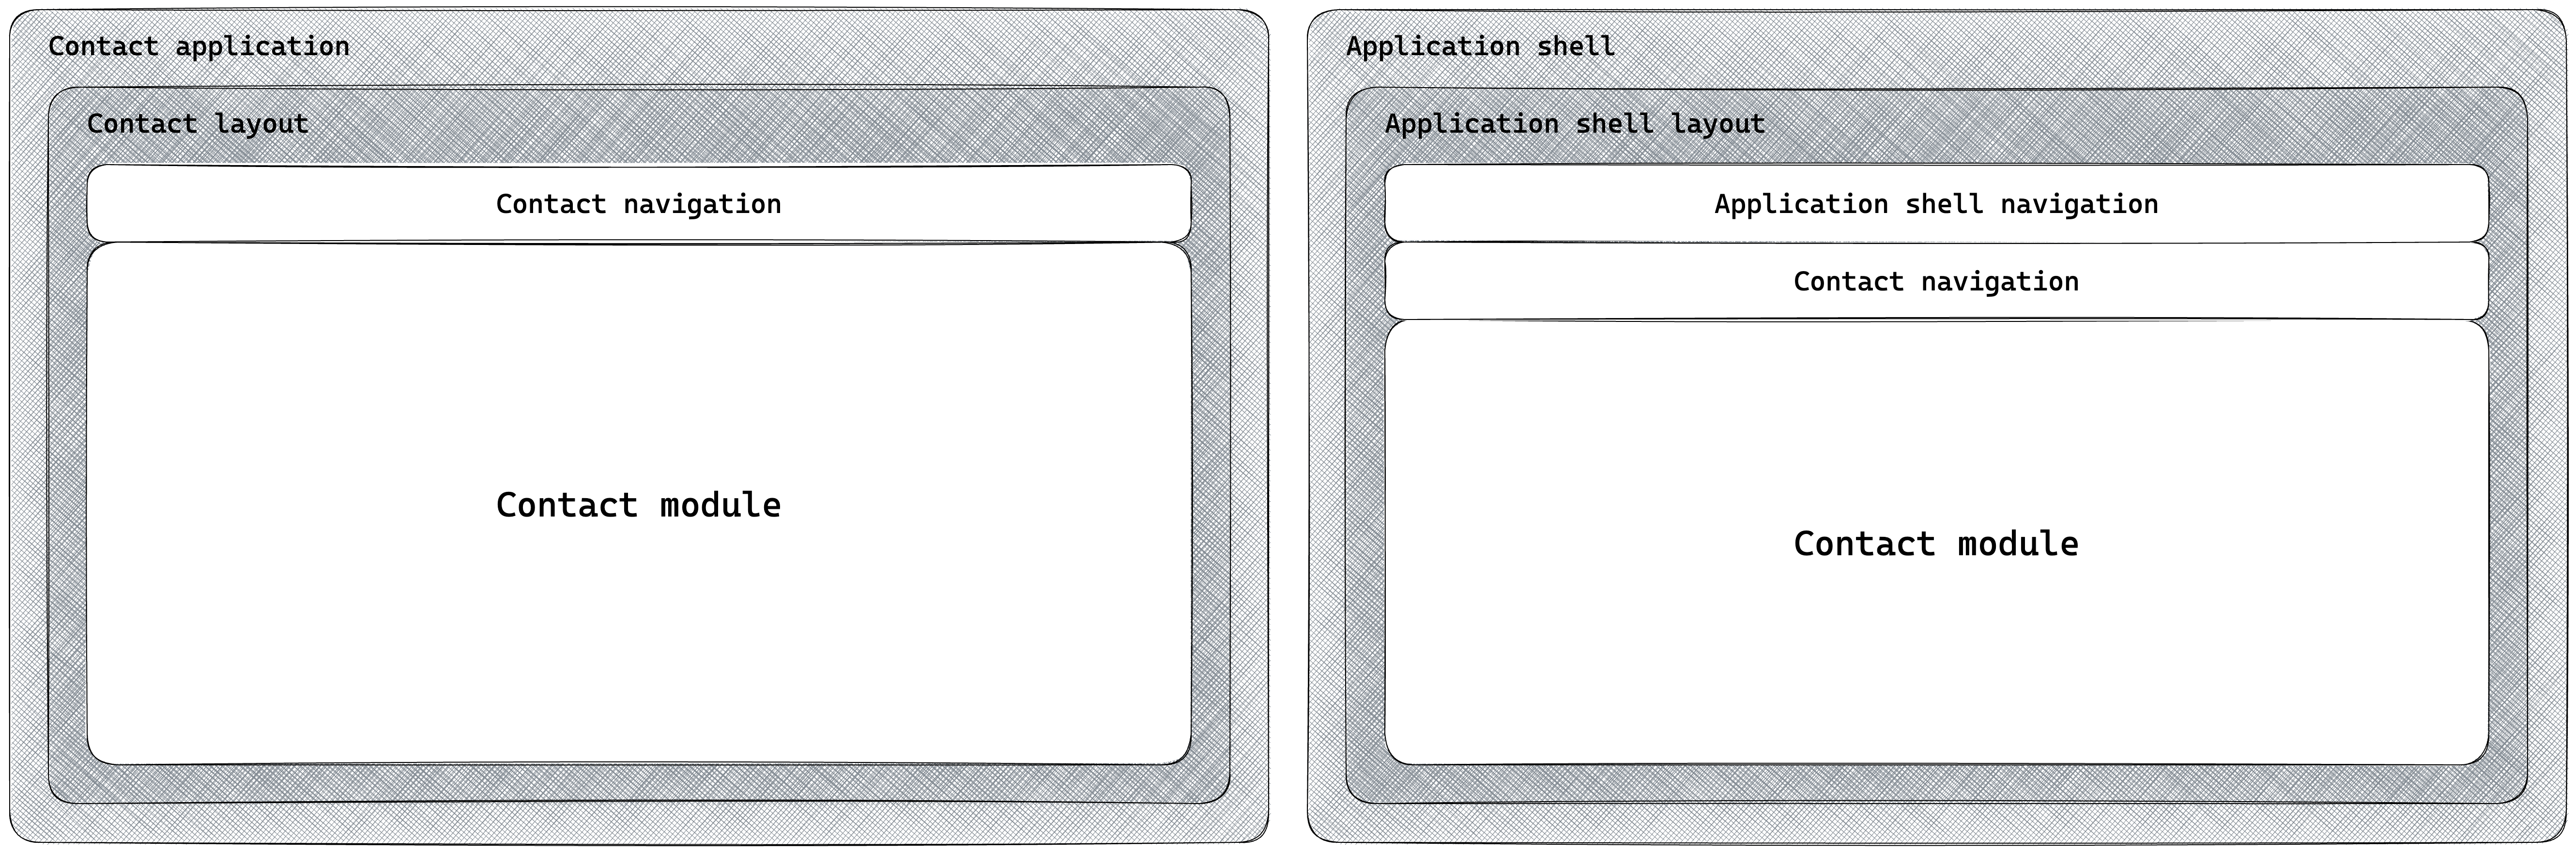
\includegraphics[width=1\linewidth]{images/applied-methods/communication-patterns/layout-comparison.png}
  \caption{Comparison between the navigation inside the contact-application and the application-shell}\label{fig:applied-methods:communication-patterns:comparison-between-host-and-contact-layout}
  \end{figure}
\fi

\noindent The application shell has to offer a mechanism to make it possible to integrate the micro-frontend into the layout. A layout service was created that can be injected into the remote modules. The layout-service navigation can register nodes in the header. The logic for registering a second row inside the toolbar is only executed if the remote module is run in a native environment. The difference between the navigation inside the application shell and the contact application can be seen in figure \ref{fig:applied-methods:communication-patterns:contact-application-header} and \ref{fig:applied-methods:communication-patterns:application-shell-header}. The first figure shows the navigation inside the contact micro-frontend to create a new contact. The second figure shows the navigation of the application shell, which incorporates the navigation of the contact micro-frontend. It has two toolbar rows. The first row is the navigation of the application shell, which links to the different micro-frontends. The second row is the navigation of the contact micro-frontend, which is only shown if the contact micro-frontend is loaded into the application shell.

\ifshowImages
  \begin{figure}[H]
  \centering
  
\includegraphics[width=1\linewidth]{images/applied-methods/communication-patterns/contact-header.png}
  \caption{The navigation inside the contact-application.}\label{fig:applied-methods:communication-patterns:contact-application-header}
  \end{figure}
\fi

\ifshowImages
  \begin{figure}[H]
  \centering
  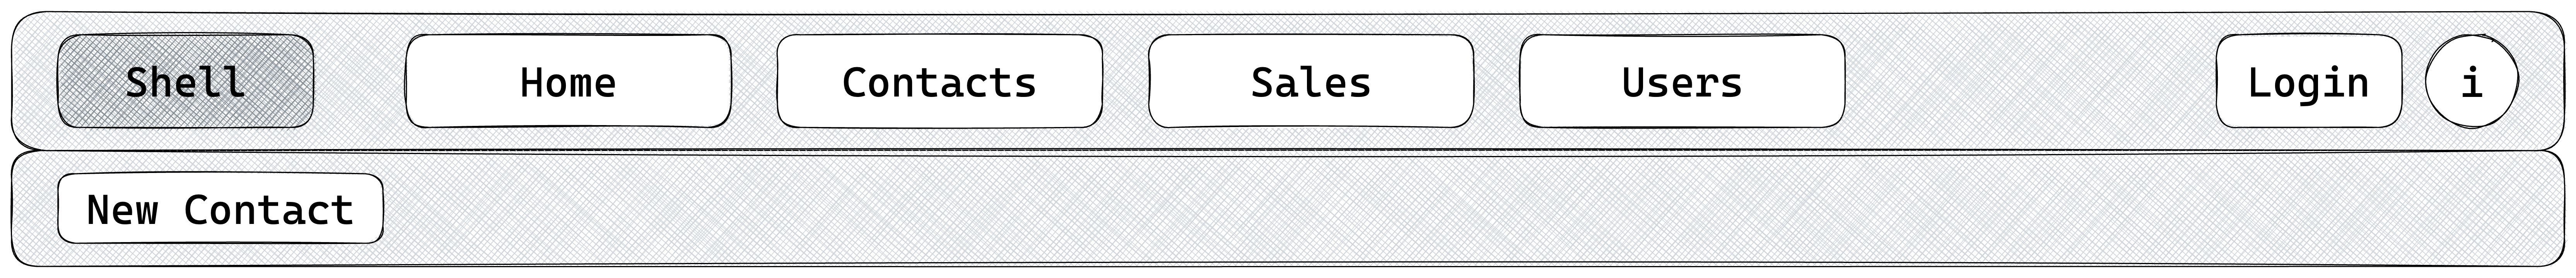
\includegraphics[width=1\linewidth]{images/applied-methods/communication-patterns/host-contact-header.png}
  \caption{The navigation of the application-shell.}\label{fig:applied-methods:communication-patterns:application-shell-header}
  \end{figure}
\fi

\noindent Some form of initialization logic has to be executed when the micro-frontend is rendered inside the application shell. This initialization logic should register the second navigation toolbar. Upon loading the micro-frontend, the second row of the navigation is registered, and it is removed upon navigating away from the micro-frontend. The initialization logic is only executed if the application is not running in a native environment. The workflow of registering and removing the second toolbar row is shown in the listing \ref{code:applied-methods:communication-patterns:initialization-logic-micro-frontend}.

\ifshowListings
  \begin{listing}[H]
  \begin{minted}{typescript}
private isNative = inject(
  CONTACT_NATIVE_ENVIRONMENT, { optional: true }
)

init() {
  const { topNodes } = CONTACT_NAVIGATION;
  if (!this.isNative)
    this.layoutService.registerSecondToolbarRow(topNodes);
}

ngOnDestroy() {
  if (!this.isNative)
    this.layoutService.unregisterSecondToolbarRow();
}
  \end{minted}
  \caption{Parts of the initialization logic of a micro-frontend}\label{code:applied-methods:communication-patterns:initialization-logic-micro-frontend}
  \end{listing}
\fi

\subsection{Layout integration}\label{subsection:applied-methods:communication-patterns:layout-integration}

At first, it was troublesome to integrate the remote module into the layout. Therefore the layout service was created with the \texttt{forRoot} and \texttt{forChild} pattern. This pattern typically provides different configuration options for a feature module.

\bigskip

\noindent Here's how it works:

\begin{itemize}
  \item The \texttt{forRoot} function is typically called in the application root module to provide configuration options for a global feature module to the entire application. This method usually returns a module with all providers available globally.
  \item The \texttt{forChild} function is called in a child module that imports the feature module to provide configuration options that are specific to that module. This method usually returns a module with providers only available to components and services within that child module.
\end{itemize}

\noindent The Listing \ref{code:applied-methods:communication-patterns:layout-module} shows the implementation of the \texttt{forRoot} and \texttt{forChild} pattern inside the layout-module.

\ifshowListings
  \begin{listing}[H]
  \begin{minted}{typescript}
class LayoutModule {
  static forRoot(): ModuleWithProviders<LayoutModule> {
    return {
      ngModule: LayoutModule,
      providers: [LayoutNavigationService, LayoutTemplateService],
    };
  }

  static forChild(): ModuleWithProviders<LayoutModule> {
    return { ngModule: LayoutModule };
  }
}
  \end{minted}
  \caption{The implementation of \texttt{forRoot} and \texttt{forChild} inside the layout module.}\label{code:applied-methods:communication-patterns:layout-module}
  \end{listing}
\fi

\noindent This approach allows the \texttt{LayoutNavigationService}- and \texttt{LayoutTemplateService}-services available in the root injector. These services can be used to register navigation nodes and templates inside the header. The \texttt{LayoutModule.forChild()} can be used where the components and directives of the layout are needed. Providing the \texttt{LayoutModule} in the root module is shown in the Listing \ref{code:applied-methods:communication-patterns:importing-the-root-layout-module}

\ifshowListings
  \begin{listing}[H]
  \begin{minted}{typescript}
@NgModule({
  imports: [ LayoutModule.forRoot() ],
})
class ContactCoreModule {}
  \end{minted}
  \caption{Provide the layout services to the root injector.}\label{code:applied-methods:communication-patterns:importing-the-root-layout-module}
  \end{listing}
\fi
